\hypertarget{implementacao-de-praticas-ageis}{%
\section{Reflexão sobre o processo de trabalho}\label{implementacao-de-praticas-ageis}}

Ao longo do desenvolvimento da plataforma de testes, esforços adjacentes foram feitos com o objetivo de melhor enquadrar o grupo de desenvolvedores em relação a práticas ágeis. Apesar deste esforço ser contínuo e ainda existirem diversas práticas ágeis a serem adotadas, é válido listar algumas já alcançadas.

\hypertarget{modelo-extreme-programming}{%
\label{modelo-extreme-programming}}
\subsubsection{Modelo Programação Extrema}

Recentemente, o grupo de desenvolvedores da colaboração entre UFRJ e \emph{CERN} vem tentando utilizar algumas práticas incentivadas pelos princípios ágeis. Condições existentes como mudança constante de requisitos e um grupo que trabalha constantemente próximo, viabilizam a adoção gradativa do modelo de \emph{Extreme Programming}. Algumas práticas já são realizadas, como reuniões semanais que são feitas com o objetivo de priorizar as funcionalidades, pequenas versões do produto que são frequentemente liberadas, e testes de aceitação que são sempre incentivados.

Em relação a organização do grupo, reuniões em pé, conhecidas como \emph{stand-up meetings}, são realizadas diariamente por todo os desenvolvedores, e a filosofia de posse coletiva é empregada internamente, na qual o código fonte não possui um único proprietário e todos têm os mesmos direitos em modificá-lo.

Práticas em pares também são encorajadas, com a recorrente \emph{pair negotiation}, na qual o par discute a melhor solução para um problema, e a ocasional \emph{pair programming}, onde a dupla implementa a solução juntos na escrita de código. O \emph{pair programming} é particularmente importante na recepção de um novo desenvolvedor, na qual se apresenta a filosofia aplicada pelos desenvolvedores do grupo durante a escrita de código.

A implementação vem sendo constantemente aprimorada. A escrita de código vem sendo padronizada com os \emph{coding standards} em conjunto com a adoção de ferramentas de verificação automática, os \emph{linters}, que serão falados mais adiante. A \emph{refatoração} é encorajada dentro do grupo, possibilitando a melhoria na clareza e na estruturação do código, e a integração contínua já é adotada nos principais repositórios. Recentemente tentativas têm sido feitas em implementar o desenvolvimento orientado a testes, conhecido como \emph{TDD}, onde se elabora primeiramente os testes unitários para depois ser implementado o código referente a estes testes. Entretanto, dada a complexidade desta abordagem, esta prática tem sido exercida apenas de forma experimental.

\hypertarget{ferramenta-de-comunicacao-interna}{%
\subsubsection{Ferramenta de comunicação interna}\label{ferramenta-de-comunicacao-interna}}

Um dos quesitos que o grupo procura sempre melhorar é a comunicação entre os desenvolvedores. Apesar dos esforços colaborativos dos desenvolvedores do grupo em serem solícitos entre si, havia a falta de uma ferramenta destinada exclusivamente ao diálogo e notificação. Foram propostas duas ferramentas como tentativa de melhoria, o \emph{Mattermost} e o \emph{Slack}. Apesar do \emph{Mattermost} ser a ferramenta recomendada no \emph{CERN}, essa não possuía notificações para dispositivos móveis, inviabilizando-a para o grupo. No fim foi decidida a adesão do \emph{Slack}.

O \emph{Slack} permite a distribuição de assuntos em diferentes canais que funcionam como \emph{chats online}, como ilustrado na figura \ref{fig:slack-example}(a). Cada participante pode escolher os canais com os quais deseja se conectar e interagir por meio de mensagens normais ou \emph{threads}. Os \emph{threads} ajudam a discutir de modo mais aprofundado um tópico específico, sem prejudicar o fluxo principal do canal. Mensagens individuais também são possíveis, assim como chamadas por conferência, e formatações para escrita de código.

Uma importante característica presente no \emph{Slack} é o suporte a comunicadores automáticos, conhecidos como \emph{bots}, exemplificado na figura \ref{fig:slack-example}(b). Os \emph{bots} são uma forma de trazer para o \emph{Slack} comunicações automáticas de serviços externos. Comunicando-se por meio de \emph{API}, se tornou possível a centralização das notificações de diversas ferramentas utilizadas pelo grupo em um só lugar. Estas notificações incluem o \emph{Gitlab} para movimentações de código, o \emph{Jira} para geração e rastreamento de entregáveis, e \emph{Confluence} para documentos criados ou editados. Desta forma, torna-se mais fácil os desenvolvedores acompanharem as mudanças, mesmo estando trabalhando remotamente.

\begin{figure}[H]
    \centering
    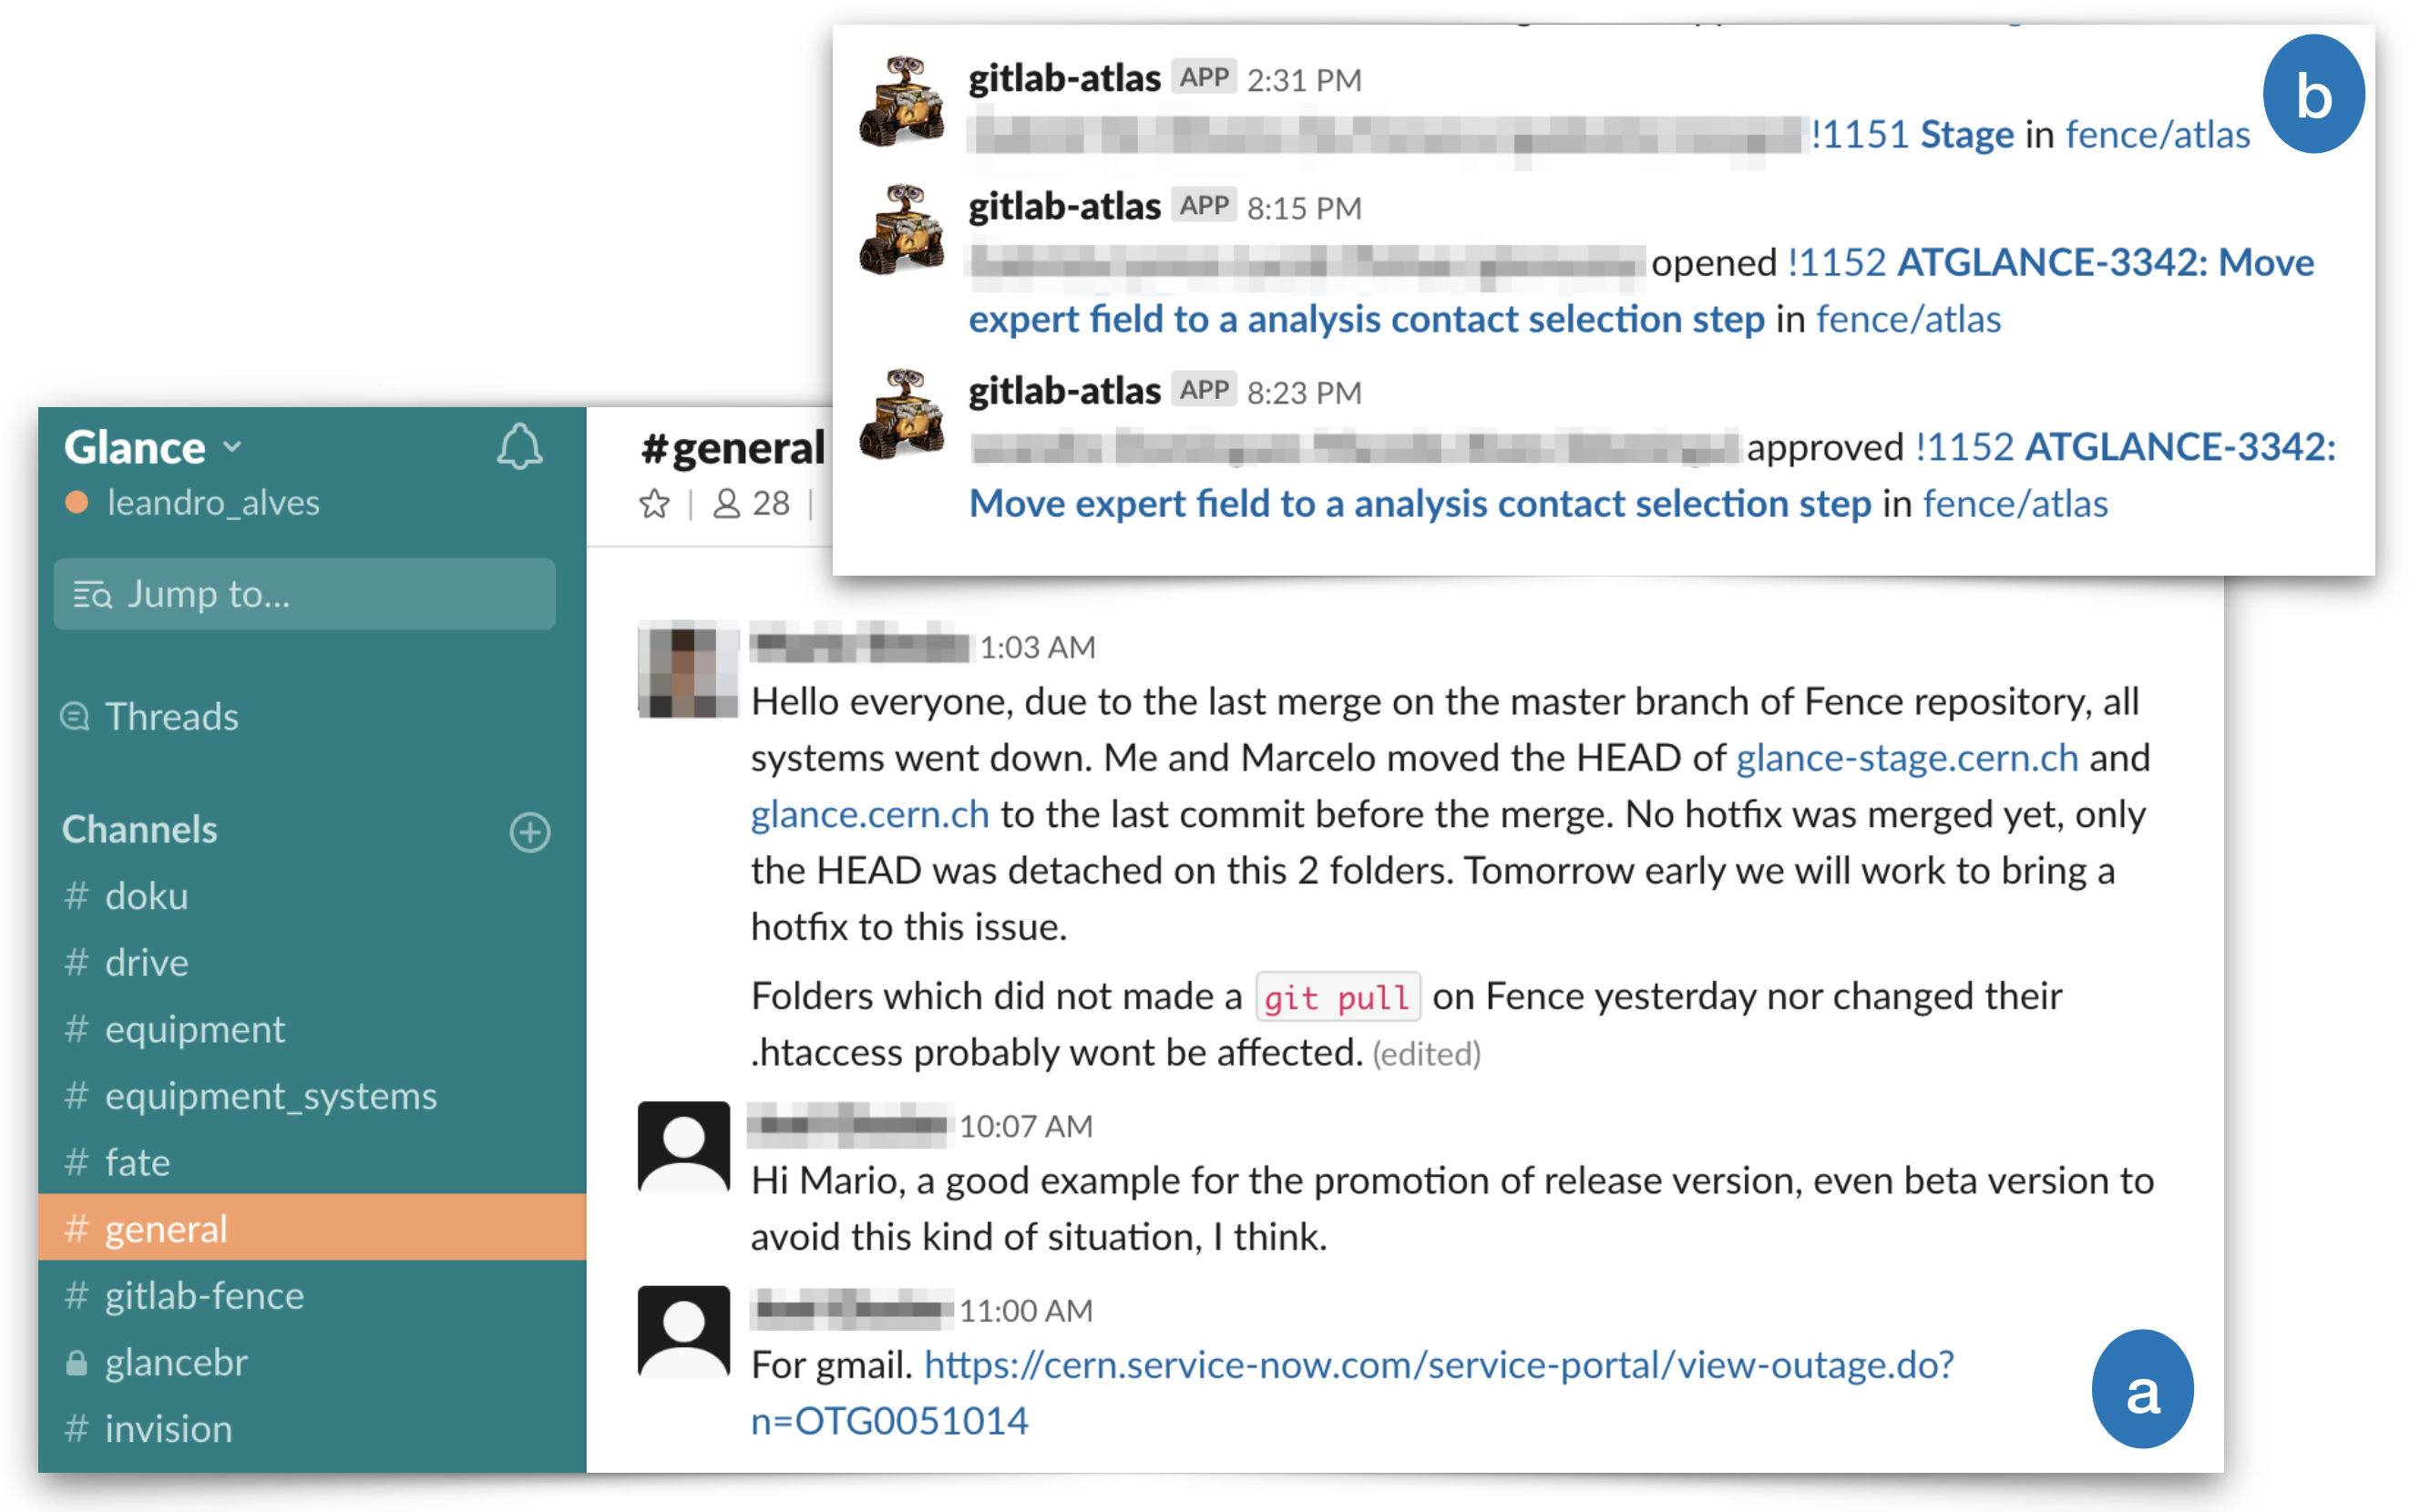
\includegraphics[width=15cm]{source/4-solucao/images/slack-example.png}
    \caption{Exibição de um canal do \emph{Slack} em $(a)$. Exemplo de mensagens geradas por \emph{bots} em $(b)$. }
    \label{fig:slack-example}
\end{figure}

\hypertarget{revisoes-de-codigo}{%
\subsubsection{Revisões de código}\label{revisoes-de-codigo}}

A contribuição mais relevante neste aspecto ágil foi a adoção da revisão de código pelo grupo, chamadas de \emph{merge requests}. Os \emph{merge requests} permitem a melhoria na comunicação entre os desenvolvedores a nível de código. Eles foram implementados nos repositórios \emph{git} do grupo, e se tratam de pedidos formais de adição de novo código às bases de código já existentes nestes repositórios. Ao realizar o pedido, o desenvolvedor deste novo código notifica por e-mail e \emph{Slack} os outros desenvolvedores responsáveis, os quais podem avaliar o conteúdo deste novo código e aprovar para poder ser inserido.

É utilizada a ferramenta web \emph{Gitlab} para gerenciamento em \emph{git} dos repositórios. Esta ferramenta proporciona uma interface para revisão de \emph{merge requests}, em que é possível realizar discussões sobre o novo código. Estas discussões podem inclusive ser apontadas em linhas de código, levantando dúvidas, sugerindo modificações ou alertando possíveis problemas, como presente na figura \ref{fig:revisao-codigo}. Depois de abertas estas discussões, o autor do \emph{merge request} pode solucioná-las ou transformá-las em \emph{issues}, que são registros de tarefas a serem realizadas posteriormente.

Uma convenção foi também adotada para melhor organizar os novos códigos desenvolvidos. Antes de começar este trabalho, é esperado que o desenvolvedor crie antes uma \emph{issue} no \emph{Jira}, contendo uma descrição deste trabalho. O \emph{Jira} é uma plataforma voltada a gerenciar os requisitos do grupo, e é a interface de contato com os usuários. Após a \emph{issue} ser gerada e seguindo o padrão do \emph{git flow}, o trabalho em código por um desenvolvedor é separado inicialmente em uma versão exclusiva, chamada de \emph{branch}. Esta versão separada permite ao desenvolvedor não afetar o trabalho dos outros e não ser afetado, e a medida que o próprio avança por meio de \emph{commits}, que são pequenas versões geradas durante a escrita de código, é possível que os observadores, ou \emph{watchers}, possam acompanhar o andamento diretamente da \emph{issue} no \emph{Jira}. Essa integração traz o usuário para mais perto do desenvolvimento em si, na tentativa de estimular a sua contribuição.

\begin{figure}[H]
    \centering
    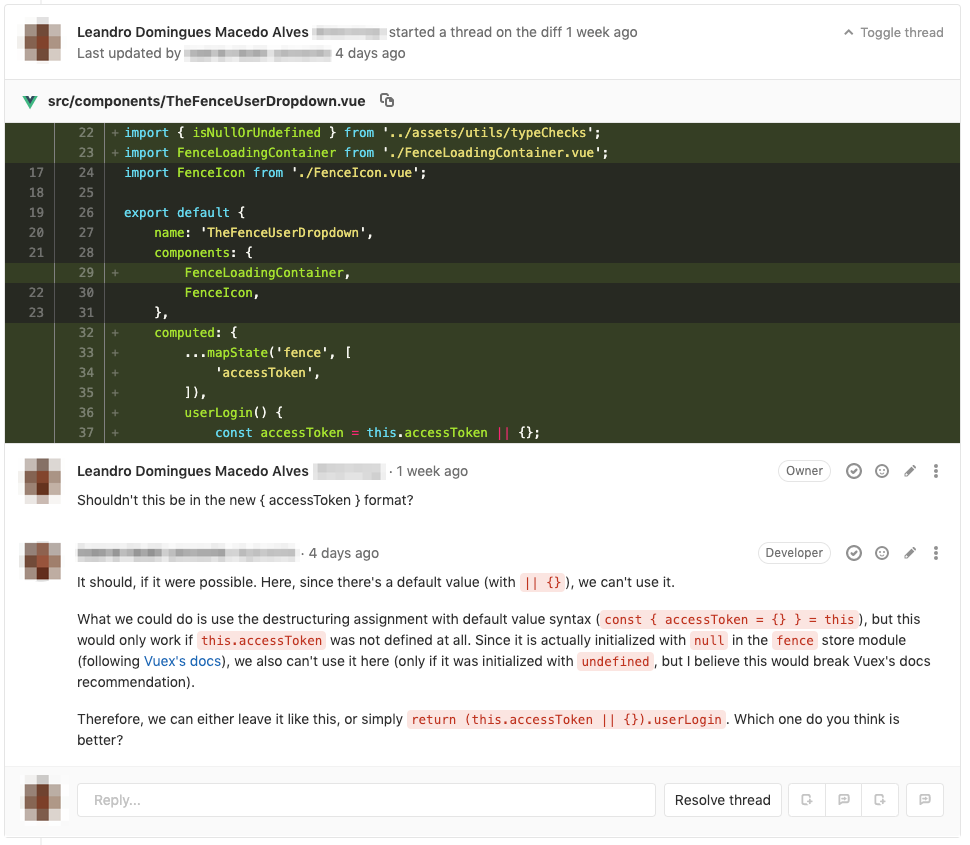
\includegraphics[width=15cm]{source/4-solucao/images/revisao-codigo.png}
    \caption{Exemplo de discussão de \emph{merge request} a partir da interface web \emph{Gitlab}.}
    \label{fig:revisao-codigo}
\end{figure}

\hypertarget{centralizacao-da-documentacao}{%
\subsubsection{Centralização da documentação}\label{centralizacao-da-documentacao}}

Sempre houve ao longo da existência do grupo de desenvolvedores a preocupação em documentar requisitos, funcionamento dos sistemas e o código fonte. Diversas ferramentas foram utilizadas, e migrações ocorreram com o passar dos anos, na tentativa constante de achar uma melhor opção, e isso consequentemente contribuiu para a dispersão da documentação entre diferentes plataformas. \emph{Google Docs}, \emph{Trac}, \emph{DokuWiki} e \emph{Twiki} estão entre elas, dificultando encontrar um documento específico, e ocorrendo a repetição de documentação. Se tornou necessário não somente achar uma ferramenta em que todo o grupo concordasse, como também realizar a migração para uma plataforma única.

Levando em consideração a satisfação do grupo com a utilização do \emph{Jira}, optou-se experimentar pela ferramenta \emph{Confluence}, ilustrada na figura \ref{fig:centralizacao-docs}(b). \emph{Confluence} possui uma integração nativa com \emph{Jira}, tornando mais fácil a referenciação a \emph{issues} durante a documentação, como a elaboração automática de relatórios semanais do trabalho feito por cada desenvolvedor, ilustrado na figura \ref{fig:centralizacao-docs}(a). Além disso, a ferramenta possui suporte a diversos \emph{plugins}, permitindo a customização para atender as especificidades do grupo, como formatações para escrita de código e \emph{templates} de atas de reunião. Após explorar a ferramenta, decidiu-se a sua adoção, e um esforço coletivo do grupo foi realizado em migrar a documentação preexistente e depreciar as antigas ferramentas.

No momento atual, o grupo se concentra em aperfeiçoar a documentação de código. Estão sendo experimentados utilitários de documentação automática para as principais linguagens usadas, como o \emph{php}, com o \emph{phpDox}, exemplificado na figura \ref{fig:centralizacao-docs}(b). O objetivo é integrar estas ferramentas no processo de trabalho com a integração contínua, e complementá-las ao \emph{Confluence}.

\begin{figure}[H]
    \centering
    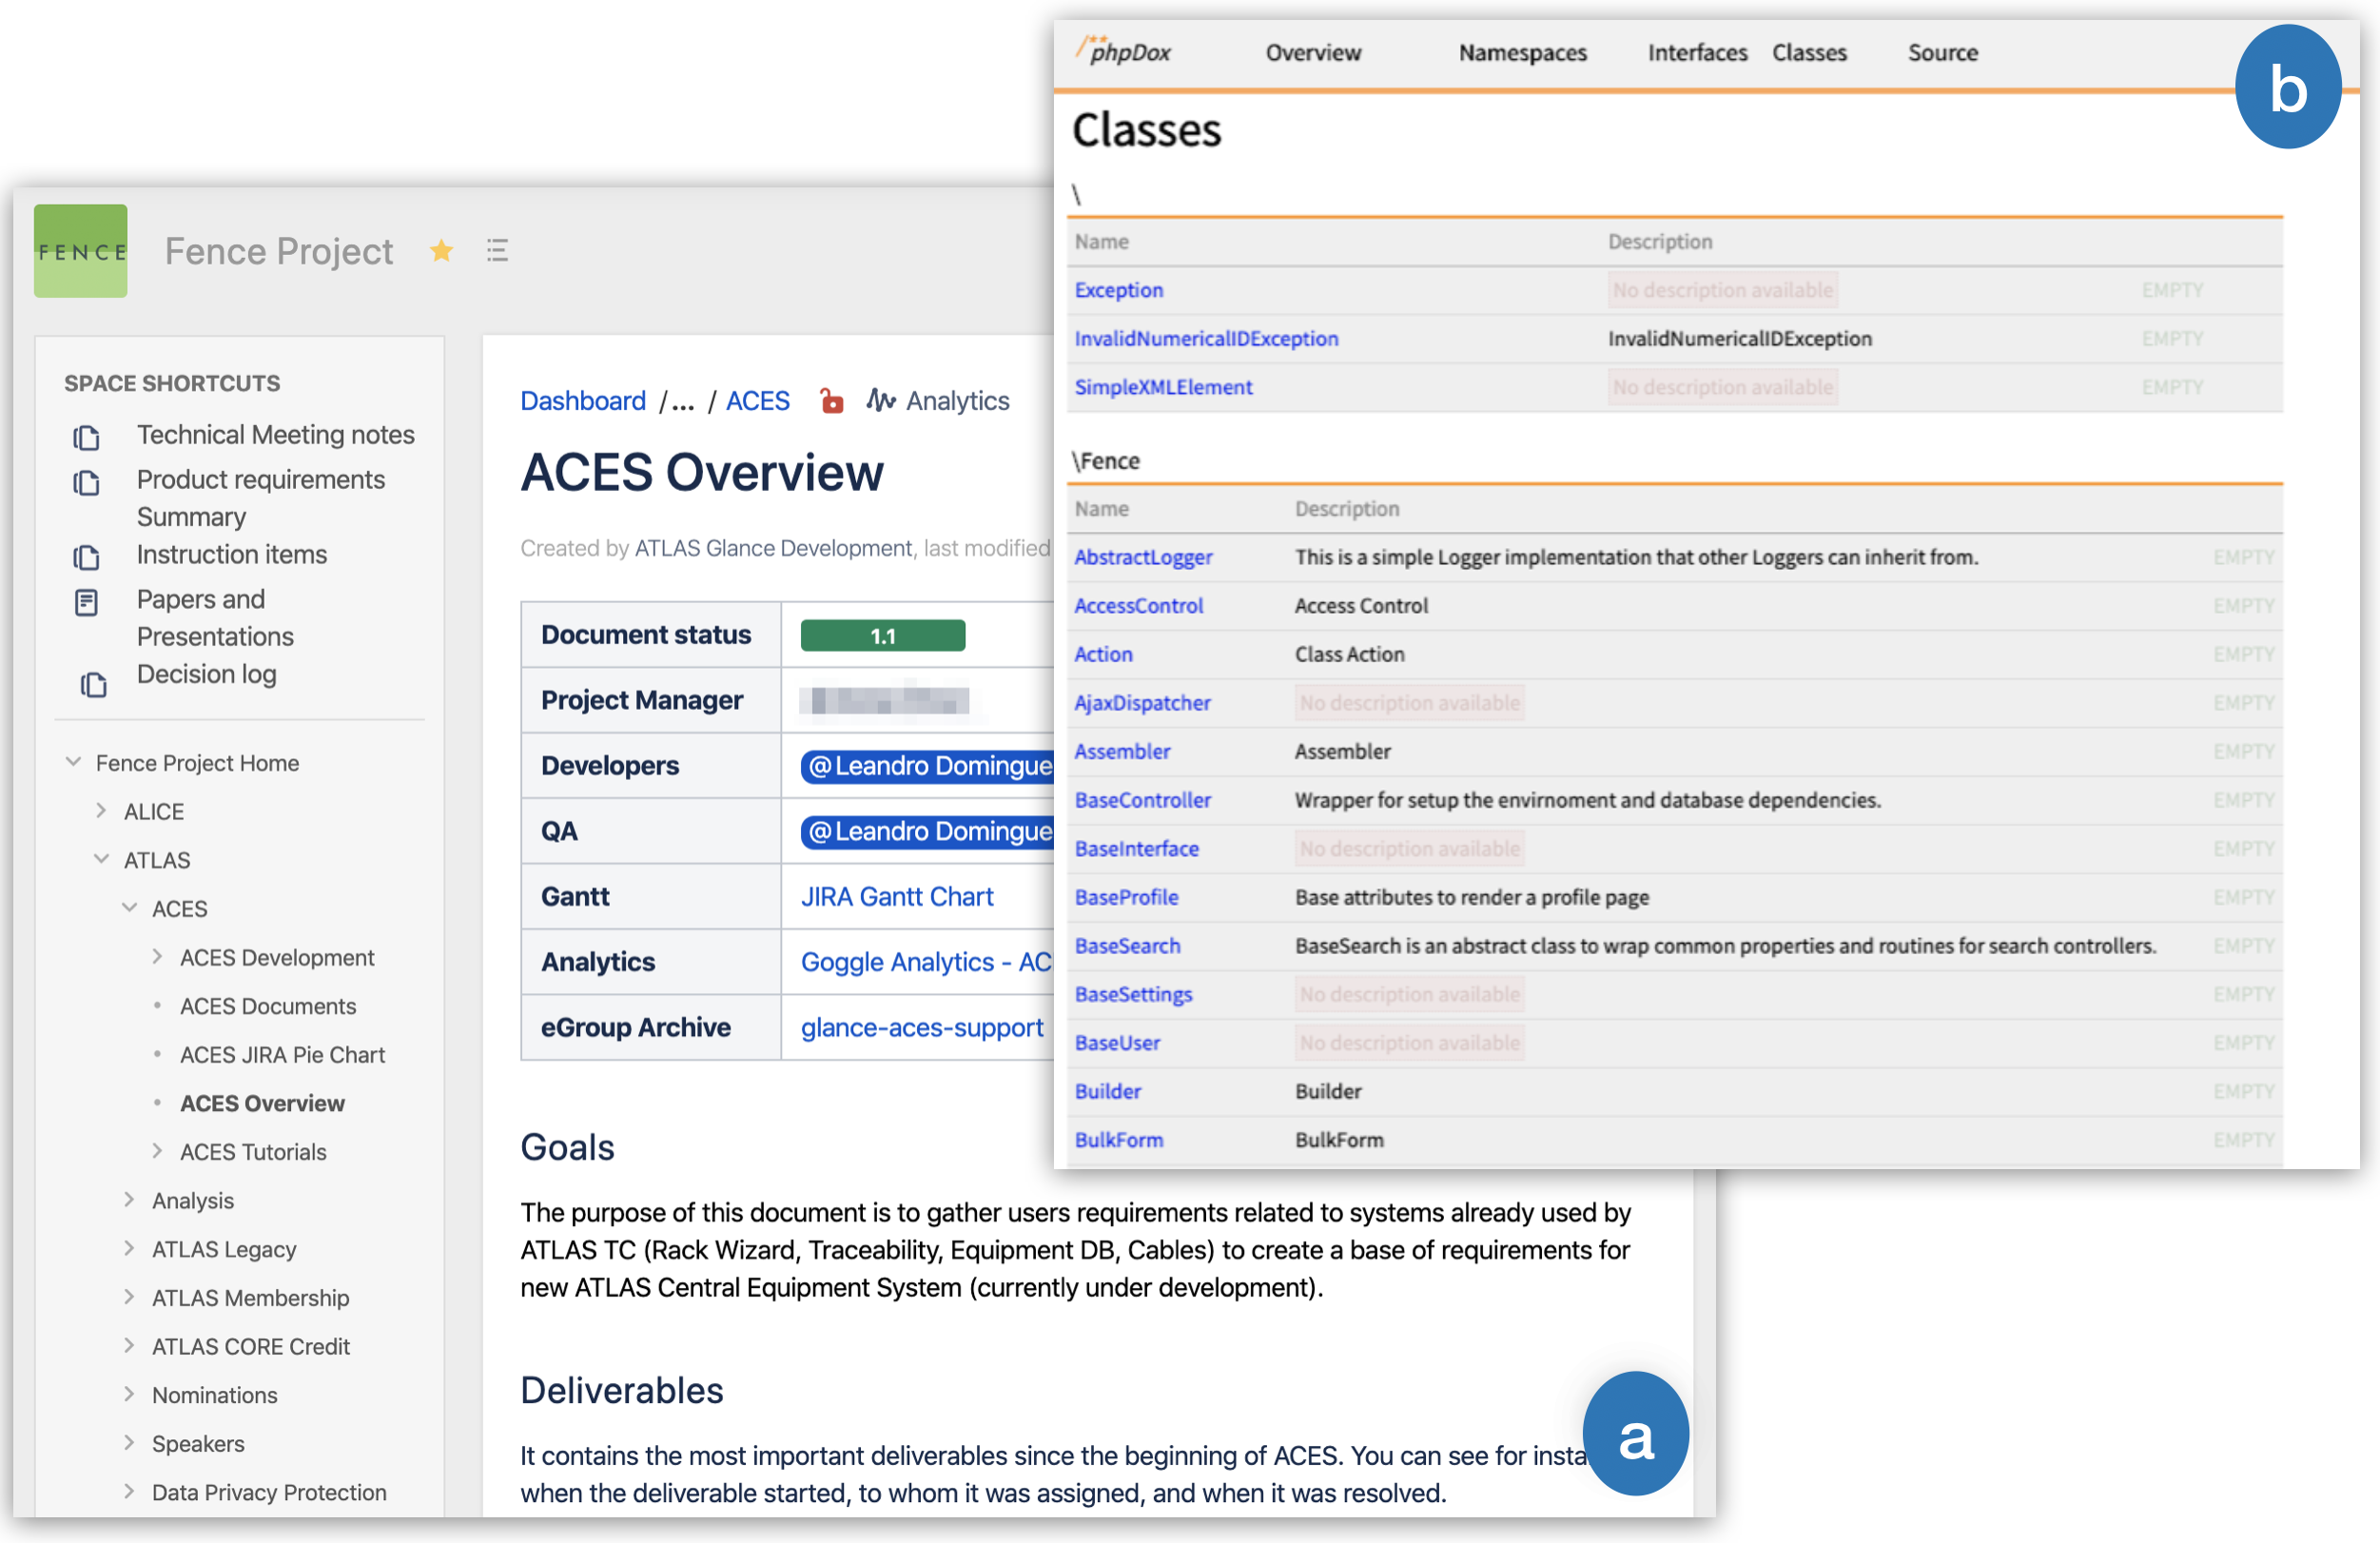
\includegraphics[width=15cm]{source/4-solucao/images/centralizacao-docs.png}
    \caption{Exemplo de documentação web elaborada a partir do \emph{Confluence} em $(a)$. Documentação automática de código gerada pelo \emph{phpDox} em $(b)$.}
    \label{fig:centralizacao-docs}
\end{figure}

Por fim, foi implementada uma integração automática entre as ferramentas de comunicação. Um documento elaborado no \emph{Confluence} possui acesso livre a \emph{issues} disponíveis na ferramenta de administração de requisitos e inconsistências \emph{Jira}. Cada \emph{issue} por sua vez possui referências ao trabalho feito em código para sua solução, com a integração à plataforma de controle de versão \emph{Gitlab}. Todas estas ferramentas enviam notificações por meio de \emph{bots} aos canais respectivos no \emph{Slack}, aonde todos os desenvolvedores possuem acesso.

\hypertarget{validadores-de-sintaxe}{%
\subsubsection{Validadores de sintaxe}\label{validadores-de-sintaxe}}

A rotatividade de pessoas sempre foi uma característica marcante dentro do grupo de desenvolvedores. Por conta desta alternância, a possibilidade de padronização de práticas sempre foi algo desejado para o grupo, inclusive em relação ao processo de escrita de código. Em geral, ocorre uma transmissão de conhecimento entre os desenvolvedores em relação a boas práticas de código, porém isto pode ser insuficiente e consumir tempo.

Levando isto consideração, foi proposta a elaboração de padrões de escrita de código, chamados de \emph{code standards}. Estes padrões são definidos em arquivos de configuração presentes nos repositórios do grupo e foram gerados para as linguagens mais utilizadas pelo grupo, sendo estas o \emph{php} e o \emph{Javascript}.

Por meio dos \emph{code standards} passou a ser utilizado pelo grupo em seus editores de código as ferramentas adicionais de análise chamadas \emph{linters}. Os \emph{linters} são capazes de aplicar as regras de \emph{code standards} durante a escrita de código, notificando o desenvolvedor de regras definidas pelo grupo e aconselhando-o de boas práticas. Desta forma, o programador ingressante tem a possibilidade de obter avaliações instantâneas sobre a qualidade de seu código, reduzindo a possibilidade de reescrita no futuro.

Atualmente são oficialmente utilizados quatro \emph{linters} na análise de código, com mais duas em fase de experimentação. Para \emph{Javascript}, somente o \emph{eslint} é utilizado para avaliar erros de sintaxe e compatibilidade com os padrões decididos. Já para \emph{php}, são utilizados o \emph{phpcs}, também para regras do grupo, o \emph{phpmd}, para principalmente análise de complexidade de métodos e classes, e o próprio validador do \emph{php}, para identificar antecipadamente potenciais erros de sintaxe. Estes \emph{linters} estão atualmente sendo utilizados nos editores de texto \emph{Sublime Text} e \emph{Visual Code}, mas também podem ser executados de forma autônoma pela linha de comando do terminal. Na figura \ref{fig:validores-sintaxe} há um exemplo de código sob revisão de \emph{linters}, de forma que as linhas que apresentam inconsistências são sublinhadas e estes erros são exibidos no compilador, contendo informações de como consertá-los.

Para garantir a consistência do uso dos \emph{linters} pelo grupo, foi disponibilizado também uma ferramenta de verificação automática chamada \emph{lint staged}. Independente se o desenvolvedor fez uso de \emph{linters} ao programar, o \emph{lint staged} é aplicado diretamente a um \emph{git hook}, de forma que estes \emph{linters} são executados durante o processo de \emph{commit}. Caso haja algum problema, o \emph{commit} é cancelado, informando as inconsistências ao desenvolvedor. Assim, evita-se a submissão por acidente de código que esteja fora do padrão do grupo ou até mesmo com erros de sintaxe.

\begin{figure}[H]
    \centering
    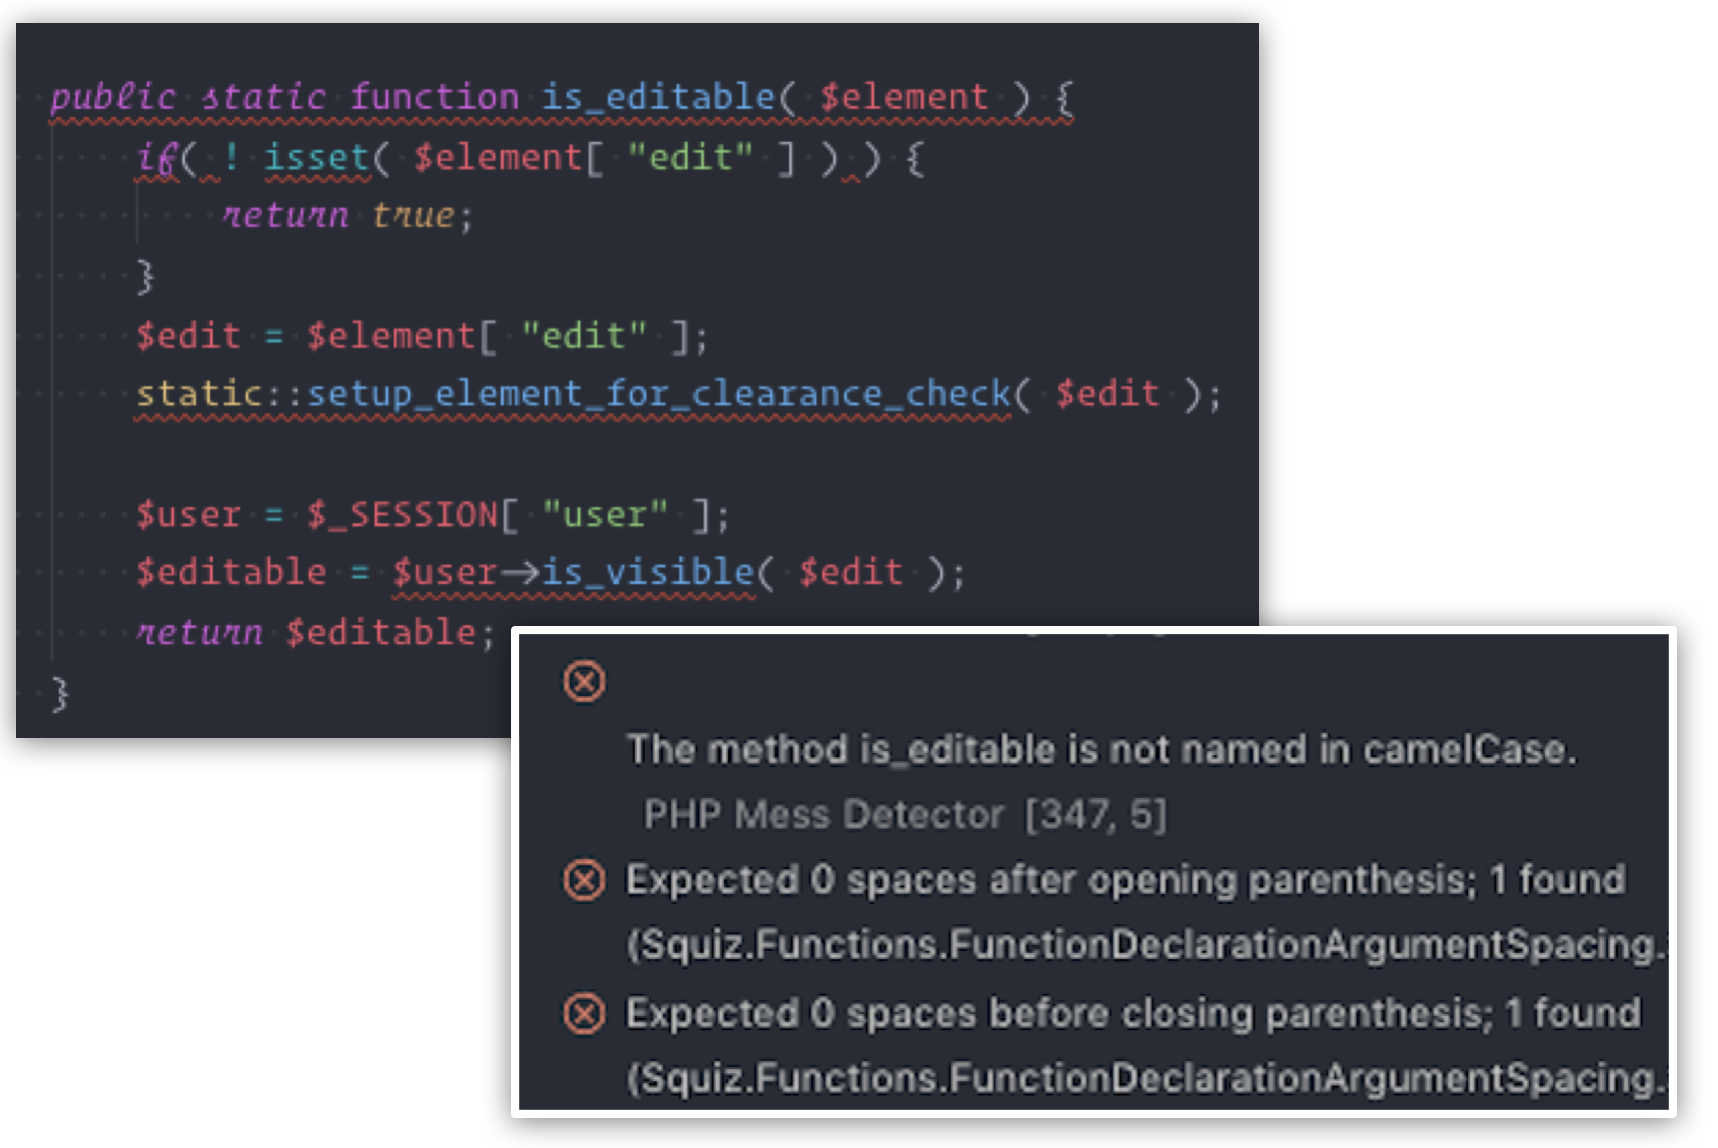
\includegraphics[width=15cm]{source/4-solucao/images/validores-sintaxe.png}
    \caption{Exemplo de alertas gerados por \emph{linters} no editor de código \emph{Visual Code}.}
    \label{fig:validores-sintaxe}
\end{figure}

\hypertarget{plano-de-testes}{%
\subsubsection{Plano de Testes}\label{plano-de-testes}}

Os desenvolvedores do grupo têm realizado a prática de planos de testes ao longo dos últimos anos, acumulando dezenas de documentos com milhares de testes. Além de contribuir para a clareza do desenvolvedor em saber o que tem que ser testado, o plano de testes também auxilia na documentação dos requisitos e na compreensão do sistema. É uma prática do grupo apresentar os planos de testes dos sistemas aos ingressantes, convidando-os a realizar testes exploratórios e de usabilidade no ambiente de desenvolvimento.

Considerando a importância do plano de testes, foi realizada uma pesquisa em busca de possíveis aprimoramentos em seu processo de desenvolvimento e manutenção, que no momento consistia em serem realizados em planilhas no \emph{Google Sheets}. Nesta pesquisa, encontrou-se uma ferramenta alternativa que se enquadra nas condições do grupo, chamada \emph{Lean Testing}. Semelhante ao \emph{Google Sheets}, o \emph{Lean Testing} permite o agrupamento de dados em diversas categorias, como \emph{test cases} e \emph{test suites}. Entretanto o \emph{Lean Testing} possui uma interface focada para as necessidades dos testadores, como a disponibilidade de histórico de execuções de testes e a possibilidade de fornecer um modelo de relatório no caso de erros. Além disso, o \emph{Lean Testing} fornece diversos gráficos sobre os resultados, facilitando uma análise qualitativa e quantitativa. Na figura \ref{fig:plano-testesfig:teste-unitario} há a ilustração das duas ferramentas contendo a listagem dos \emph{test cases}.

\begin{figure}[H]
    \centering
    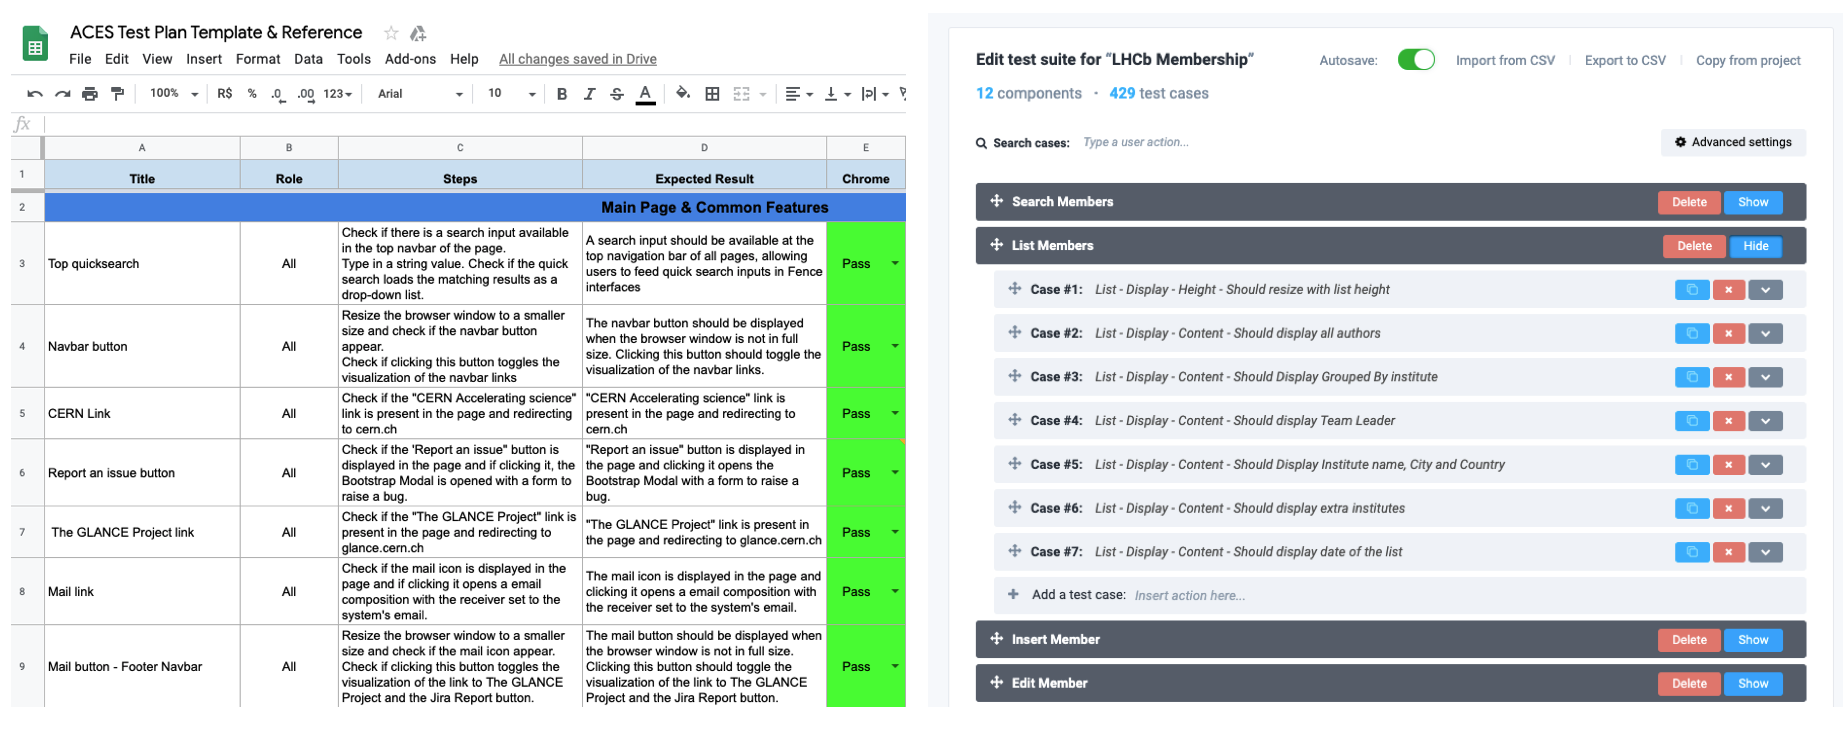
\includegraphics[width=15cm]{source/4-solucao/images/plano-testes.png}
    \caption{Exemplo de plano de testes feito através do \emph{Google Sheets} à esquerda e \emph{Lean Testing} à direita.}
    \label{fig:plano-testesfig:teste-unitario}
\end{figure}

Este capítulo abordou as principais contribuições deste trabalho para o processo de desenvolvimento do grupo. Inicialmente foi falado sobre o desenvolvimento de duas ferramentas de testes orientadas a contribuir para a escrita de testes, com o \emph{FUnit} direcionado para testes unitários e o \emph{Fate} para testes \emph{e2e}. Após isso foi abordada a estratégia adotada para administração automática destas ferramentas, aprimorando o processo de trabalho dos desenvolvedores. Por fim foi debatido o esforço na adoção de práticas ágeis dentro da cultura do grupo, com o objetivo de melhorar a qualidade das entregas. No próximo capítulo será apresentado os resultados obtidos com o trabalho desenvolvido e uma análise será feita em relação a estes resultados.